\documentclass[a4paper, 11pt]{article}
\usepackage{graphics,graphicx}
\oddsidemargin=-0.54cm
\evensidemargin=-0.54cm
\topmargin=-1.2cm
\textwidth=17cm
\textheight=25cm
\pagestyle{empty}
    \usepackage[
    top    = 3.0cm,
    bottom = 2.0cm,
    left   = 2.5cm,
    right  = 2.2cm]{geometry}
\begin{document}

\section{Abstract}
Astronomical observations have shown that black holes exist at two different mass scales -- stellar--mass black holes formed from the collapse of dying stars, and so--called {\it supermassive} black holes fed by the accretion of gas into the central regions of galaxies. While theoretical mechanisms for the formation of black holes at intermediate mass scales have been proposed, the empirical evidence for such objects has remained scant. However, the potential of exploiting effects due to gravitational lensing -- the bending of light by strong gravitational fields -- to hunt these objects down has so far been largely unexplored.
Gravitational lensing has already allowed astronomers to find planets outside our solar systems, to estimate the masses of galaxies and probe the dark matter of the Universe. Our team has singled out a gravitationally lensed radio jet with properties that appear consistent with our simulations of lensing by an intermediate mass-black hole, and were granted in total 24 hours of time with the European (PI Zackrisson) and global (PI Asadi) very long baseline interferometry (VLBI) arrays to test our hypothesis. Previous maps of the gravitationally--lensed quasar in B1152+199 with lower angular resolution have resulted in a tentative detection of a dark compact substructure in the main lens with mass 10$^5$--10$^7$ M$_\odot$, based on the jet curvature seen in one of the two macroimages in this system. We are now in possession of three unpublished observations of the system B1152+199, in the frequency range between 1.4\,GHz to 22\,GHz. Our plan for the project is to {\bf A)} confirm the jet curvature and {\bf B)} search for previously unresolved distortions in the curved jet to provide the first robust detection of secondary gravitational lensing by a compact dark object in the system. Our numerical models suggest that if the peculiar appearance of this radio source is indeed due to gravitational lensing by a foreground object, then that object must have properties very similar to an intermediate--mass black hole. If confirmed, this would not only be the smallest gravitational lens ever discovered, but also the first case of a black hole discovered through gravitational lensing, at any mass scale.

\section{Gravitational lensing and black holes}
Rays of light do not always follow straight paths. Gravitational lensing is a well-known effect in astronomy, by which overdensities of matter along the line of sight cause a bending in the light from distant light sources. The size of this effect was accurately predicted by Einstein in 1915, and has in the last few decades helped astronomers to detect free--floating exoplanets, to estimate the masses of galaxies and galaxy clusters, to measure cosmological parameters and constrain the nature of dark matter (for a review, see Bartelmann 2010). Secondary gravitational lensing effects are also used to probe overdensities inside the primary lens (i.e. galaxies in galaxy clusters or dwarf galaxies in galactic lens systems). Figure 1 features a schematic example of a secondary gravitational lensing effect, in which an overdensity inside the main lens (galaxy) happens to lie in the line of sight of one of the images made by the main lens. The overdensity causes a small--scale perturbation in the spacetime at the position of one of the images. This distorts that lensed image of the background light source without affecting the other images, which makes it possible to distinguish the secondary lensing effect from morphological peculiarities that may be present within the source.

\begin{figure}[tbh]
\centering
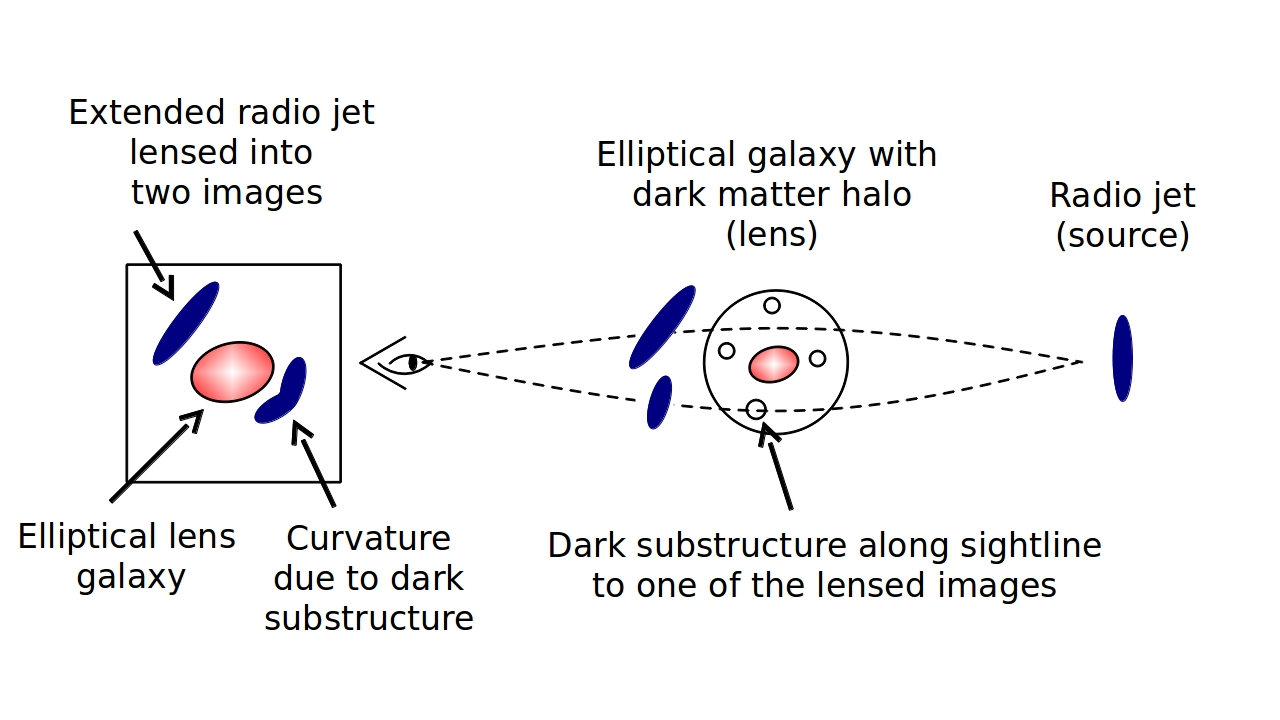
\includegraphics[scale=0.3]{Figure-lensing-v3.jpg}
\caption{Schematic illustration of gravitational millilensing as a probe of the local overdensity (a dwarf galaxy, a dark matter subhalo, or a black hole). A foreground galaxy with a dark matter halo produces two images of a background light source (macroimages). An intermediate--mass black hole (IMBH) located in the dark halo intercepts the path of one of these macroimages and produces a small--scale distortion (millilensing) in its surface brightness distribution. Whereas morphological anomalies intrinsic to the source should be mimicked in both macroimages, millilensing will affect each macroimage differently, and typically turn up just in one image.}
\end{figure}

The angular scale of the distortion depicted in Figure 1 is primarily determined by the mass of the secondary lens. A galaxy--mass lens gives rise to a ring with a radius of order one arcsecond (1/3600 of a degree). Objects of intermediate--mass black hole scale are expected to give rise to lensing effects on sub--milliarcsecond scales, and current radio interferometers are in principle able to resolve such structures down to 0.05--1 milliarcsecond (mas). Even so, secondary lensing effects of the type depicted in Figure 1 made by intermediate--mass black holes (IMBH) have -- until now -- not been confirmed. The proposed project revolves around a potential detection of an unusual curvature in one of the images of an already lensed quasar jet -- the very first case of its kind. Lensing effects at this scale can be produced either by very compact forms of matter such as black holes, or objects with lower mass concentrations such as dark matter subhalos (e.g. Zackrisson \& Riehm 2010, Zackrisson et al. 2013). However, only objects in the former category are sufficiently compact to produce distinct lensing features on radio jets (Zackrisson et al. 2013). 

Astronomers already have strong observational evidence for the existence of black holes at two different mass scales (for a review, see Narayan \& McClintock 2013): Stellar--mass black holes (5--30 times the mass of the Sun) and supermassive black holes ($\sim$ 10$^6$ -- 10$^9$ times the mass of the Sun). It has been postulated that intermediate--mass black holes ($\sim$ 10$^2$ -- 10$^6$ times the mass of the Sun) could form from the collapse of the central regions of star clusters (e.g. Portegies Zwart et al. 2004), from the collapse of very massive stars (e.g. Freese et al. 2010) or from direct collapse of gas clouds in the early Universe (e.g. Yue et al. 2014), but the empirical evidence for such black holes remains controversial (see Kormendy \& Ho 2013 for a review). If the mass of the object responsible for the lensing in our target object can be accurately pinned down to lie in the $\sim$ 10$^2$ -- 10$^6$ Solar mass range, this would hence have important implications for our understanding of the cosmic mass distribution of black holes.

\section{The case of secondary gravitational lensing at sub--milliarcsecond scales}
Our team has had a long--vested interest in hunting down cases of gravitational lensing on milliarcsecond/sub--milliarcsecond scales (Zackrisson et al. 2008, Riehm, Zackrisson et al. 2009, Zackrisson \& Riehm 2010, Zackrisson et al. 2013). By going through archival data from various high--resolution radio interferometers, we have come across a candidate for such small--scale gravitational lensing. The object in question, B1152+199, is a strong lensing system, discovered as part of the Cosmic Lens All--Sky Survey (CLASS), consisting of a quasar's radio jet at z = 1.019 lensed by a single galaxy at z = 0.439 into two images which are 1".56 apart in the sky (Myers et al. 1999). The single--lens model of the system, based on 5\,GHz VLBA maps of the blazar as well as {\it I}-- and {\it V}--band HST images (Rusin et al. 2002), was shown to be insufficient to explain the anomalous curvature in image B (see Figure 2, right panel). Metcalf (2002) suggested that the curvature in image B is was due to one (or more) compact perturber(s) of mass $\sim10^5$--$10^7 h^{-1} M_\odot$ along the line of sight to image B. However, the resolution of the data at 5\,GHz ($\sim3$\,mas where image B is only $\sim15$\,mas long) barely allows further constraints on the mass and inner structure of the perturber(s).

%% Metcalf's figure
\begin{figure}[tbh]
\centering
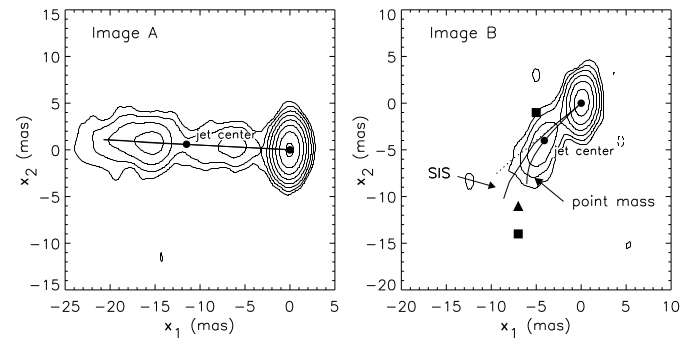
\includegraphics[scale=0.75]{Figure-2002.jpg}
\caption{The VLBA 5-GHz maps (Rusin et al. 2002) of the two macroimages of B1152+199, overlaid with lens models from Metcalf (2002). The slight curvature of the jet in the right panel (image B) is attributed to millilensing by a secondary lens located close to this macroimage. In the absence of such small--scale lens, the jet in the right macroimage would follow the path given by the dotted, straight line (a poor fit to the data). The two curved paths are produced when different forms of substructures are introduced. The lowermost curve is given by a point-mass substructure (a black hole) of mass $\sim 10^5$–-$10^7 M_\odot$ located at the position of the triangle. The intermediate curve is reproduced by two singular isothermal spheres (squares) with poorly constrained masses. Metcalf (2002) emphasizes that while the jet bending indicates some form of millilensing, the substructure solution (in terms of substructure position and mass) to these data is by no means unique.}
\end{figure}


\section{Project description}

\subsection{Scientific impact}
If B1152+199 could be established as a case of milliarcsecond-scale gravitational lensing, this would by itself be n extraordinary discovery. The fact that this could also be the first--ever case of an intermediate--mass black hole detected through gravitational lensing makes the case even more tantalizing. However, to make the case that the curved jet structure of this object is indeed caused by the bending of light by a massive foreground object requires dedicated gravitational lens modeling, which we are hereby attempting to secure funding for.

%% Our 5 GHz data
\begin{figure}[tbh]
\centering
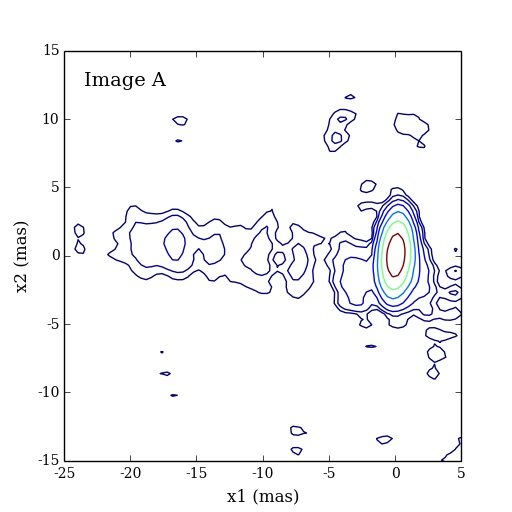
\includegraphics[scale=0.35]{imageA.jpg}
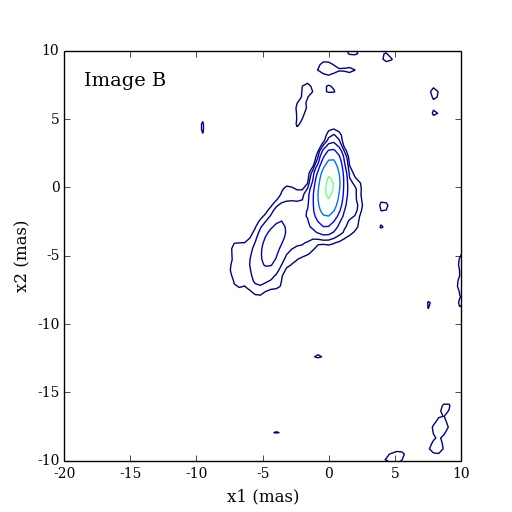
\includegraphics[scale=0.35]{imageB.jpg}
\caption{The archival EVN 5-GHz maps of the two macroimages of B1152+199. Contour levels are the same as in figure 2; the lowest contour is 3 times the map rms noise in figure 2 ($75 \mu$ Jy beam$^{-1}$) and each contour level increases by a factor of 2. The slight curvature of the jet in the right panel (image B) seems to be unchanged over 10 years. This, in addition to the much shorter ($\approx 40$--$70$ days) gravitational time delay of the system, suggests that the curvature cannot be due to jet precession.}
\end{figure}

\subsection{Data and interpretation}
The B1152+199 radio source belongs to a class of objects known as active galactic nuclei, which at radio frequencies -- in the absence of gravitational lensing -- typically appear as bright cores with one or two jets emerging from their central regions. This object has also been observed by powerful radio arrays at four different frequency bands covering 1.4\,GHz to 22\,GHz, as well as the Hubble Space Telescope (Rusin et al. 2002). Already in 2001, the unusual curvature in one of the images of the system was noted by Metcalf (2001), and Rusin et al. (2002). They, however, admitted that certain conclusions about the presence and nature of the potential secondary lens in the system would only be possible if higher resolution images of the system were available. Now, we have access to an archival dataset of the system with a time difference of about 10 years. This is enough time difference to rule out intrinsic source variabilities for such a system with significant variation over time scale of a few months. The preliminary analysis of the archival 5\,GHz data set indicates a persisting curvature in image B (Figure 3). Therefore, given the 10--year time difference between the two data sets, and the much shorter variation time scale of jet blobs, the (milli)lensing nature of the jet curvature seems to be confirmed. Our group also made an attempt to observe the same target at a higher frequency band with the global VLBI array (PI Asadi), improving the angular resolution by a factor of $\sim$ 9. Preliminary analysis of all three datasets of the system -- with 2 different frequency bands covering a period of $\sim$ 15 years -- persistently show an anomaly in the system. Comparing the results of our previous computer simulations of similar systems (Zackrisson et al. 2013) with the observational evidence in B1152+199, we expect to be able to constrain the position and mass of the potential IMBH in this system.

\subsection{Project timeline}
We estimate that it would take about 5 months of full--time work to apply our computer-- based model of gravitational lensing (Zackrisson et al. 2013) to confirm or falsify the gravitational lensing interpretation of B1152+199 by an intermediate--mass black hole or another compact object in the same mass range. I am a fourth-year PhD student and I am planning to spend this time after finishing my PhD in the end of summer 2016, as I have been leading the observational part of the project, and worked on the preliminary data analysis so far.

\subsection{Team}
Our team consists of:
\begin{itemize}
\item Saghar Asadi (4$^\mathrm{th}$ year PhD student at Stockholm University -- main applicant), with project title ``Gravitational lensing and radio interferometry as a probe of the small--scale structure of dark matter''. I have previous experience of simulations of gravitationally--lensed objects with secondary lens effects due to small--scale structures of dark matter with radio interferometers such as the Atacama Large Millimeter/sub--millimeter Array (ALMA). I have also been working with the archival data on B1152+199, based on which I lead the observing proposal that was granted time at the global VLBI array in 2015.
\item Erik Zackrisson (Associate Professor at Uppsala University), with ample experience in the field of gravitational lens modeling. Erik Zackrisson was recruited by Uppsala University in 2015 to take over leadership of the Galaxies and Cosmology research group at the Department of Physics and Astronomy after the recent retirement of Professor Nils Bergvall.
\end{itemize}

\section*{References}
\begin{itemize}
\item Bartelman, M. 2010, Gravitational lensing, Classical and Quantum Gravity, Volume 27, 233001
\item Freese, K., et al. 2010, Supermassive Dark Stars: Detectable in JWST, Astrophysical Journal, 716, 1397
\item Kormendy, J. Ho, L. C. 2013, Coevolution (Or Not) of Supermassive Black Holes and Host Galaxies, Annual Review of Astronomy and Astrophysics, 51, 511
\item Metcalf, R. B. 2002, The Detection of Pure Dark Matter Objects with Bent Multiply Imaged Radio Jets ,Astrophysical Journal, 580, 696
\item Narayan, R., McClintock, J. E. 2013, Observational Evidence for Black Holes, in General Relativity and Gravitation: A Centennial Perspective", Editors: A. Ashtekar, B. Berger, J. Isenberg and M.A.H. MacCallum, Cambridge University Press (open access link: http://arxiv.org/abs/1312.6698)
\item Portegies Zwart, S. F., et al. 2004, Formation of massive black holes through runaway collisions in dense young star clusters, Nature, 428, 724
\item  Riehm, T., Zackrisson, E., et al. 2009, Strong Lensing by Subhalos in the Dwarf-galaxy-mass Range. II. Detection Probabilities, Astrophysical Journal 700, 1552
\item  Rusin, D., et al. 2002, High-resolution observations and mass modelling of the CLASS gravitational lens B1152+199, Monthly Notices of the Royal Astronomical Society, 330, 205
\item  Yue, B., et al. 2014, The brief era of direct collapse black hole formation, Monthly Notices of the Royal Astronomical Society, 440, 1263
\item  Zackrisson, E. et al. 2008, Strong Lensing by Subhalos in the Dwarf Galaxy Mass Range. I. Image Separations, Astrophysical Journal 684, 804
\item  Zackrisson, E. \& Riehm, T. 2010, Gravitational Lensing as a Probe of Cold Dark Matter Subhalos (invited review), Advances in Astronomy, 478910
\item  Zackrisson, E., et al. 2013, Hunting for dark halo substructure using submilliarcsecond-scale observations of macrolensed radio jets, Monthly Notices of the Royal Astronomical Society 431, 2172
\end{itemize}
\end{document}
